\cleardoublepage
\section{Mathematical model}
\label{sec:mathMod}
In the present work, the air-flow in the inhabited area is investigated together with the transport of the pollution emerging on the main road. The chosen simulation approach is a segregated one: 
\begin{inparaenum}[(i)]
    \item a steady state velocity field is pre-calculated using Navier-Stokes equations, and
    \item it is used in scalar transport equation to simulate advancement of the pollution. 
\end{inparaenum}

The present section describing the used mathematical model is structured as follows: 
\begin{inparaenum}[(i)]
    \item a model geometry and a computational mesh generation are presented,
    \item used boundary conditions are summarized and
    \item the governing equations are briefly outlined.
\end{inparaenum}

\subsection{Model geometry generation and boundary conditions}
\label{subsec:geomGen}
As stated, the air flow and the spread of the pollution in the inhabited area is of an interest. A studied part of the city is $L_{\mathrm{l}} = 500$\,m long, $L_{\mathrm{w}} = 500$\,m wide, and the highest building is $L_{\mathrm{h}} = 105$\,m tall. The available \textit{stl} file together with its dimensions and the orientation in the chosen Cartesian coordinate system is depicted in Figure~\ref{fig:geom1}.

\begin{figure}[htpb]
    \begin{tikzpicture}[
            axPic/.pic={
                \draw[->,-triangle 45] (0,0) -- (-0.,0.8)  node (ysign) [pos=1,right] {$z$};
                \draw[->,-triangle 45] (0,0) -- (0.5,0.33) node (xsign) [pos=1,right] {$x$};
                \draw[->,-triangle 45] (0,0) -- (-0.6,0.2) node (zsign) [pos=1,left] {$y$};
            }]
            
        \node (obr) {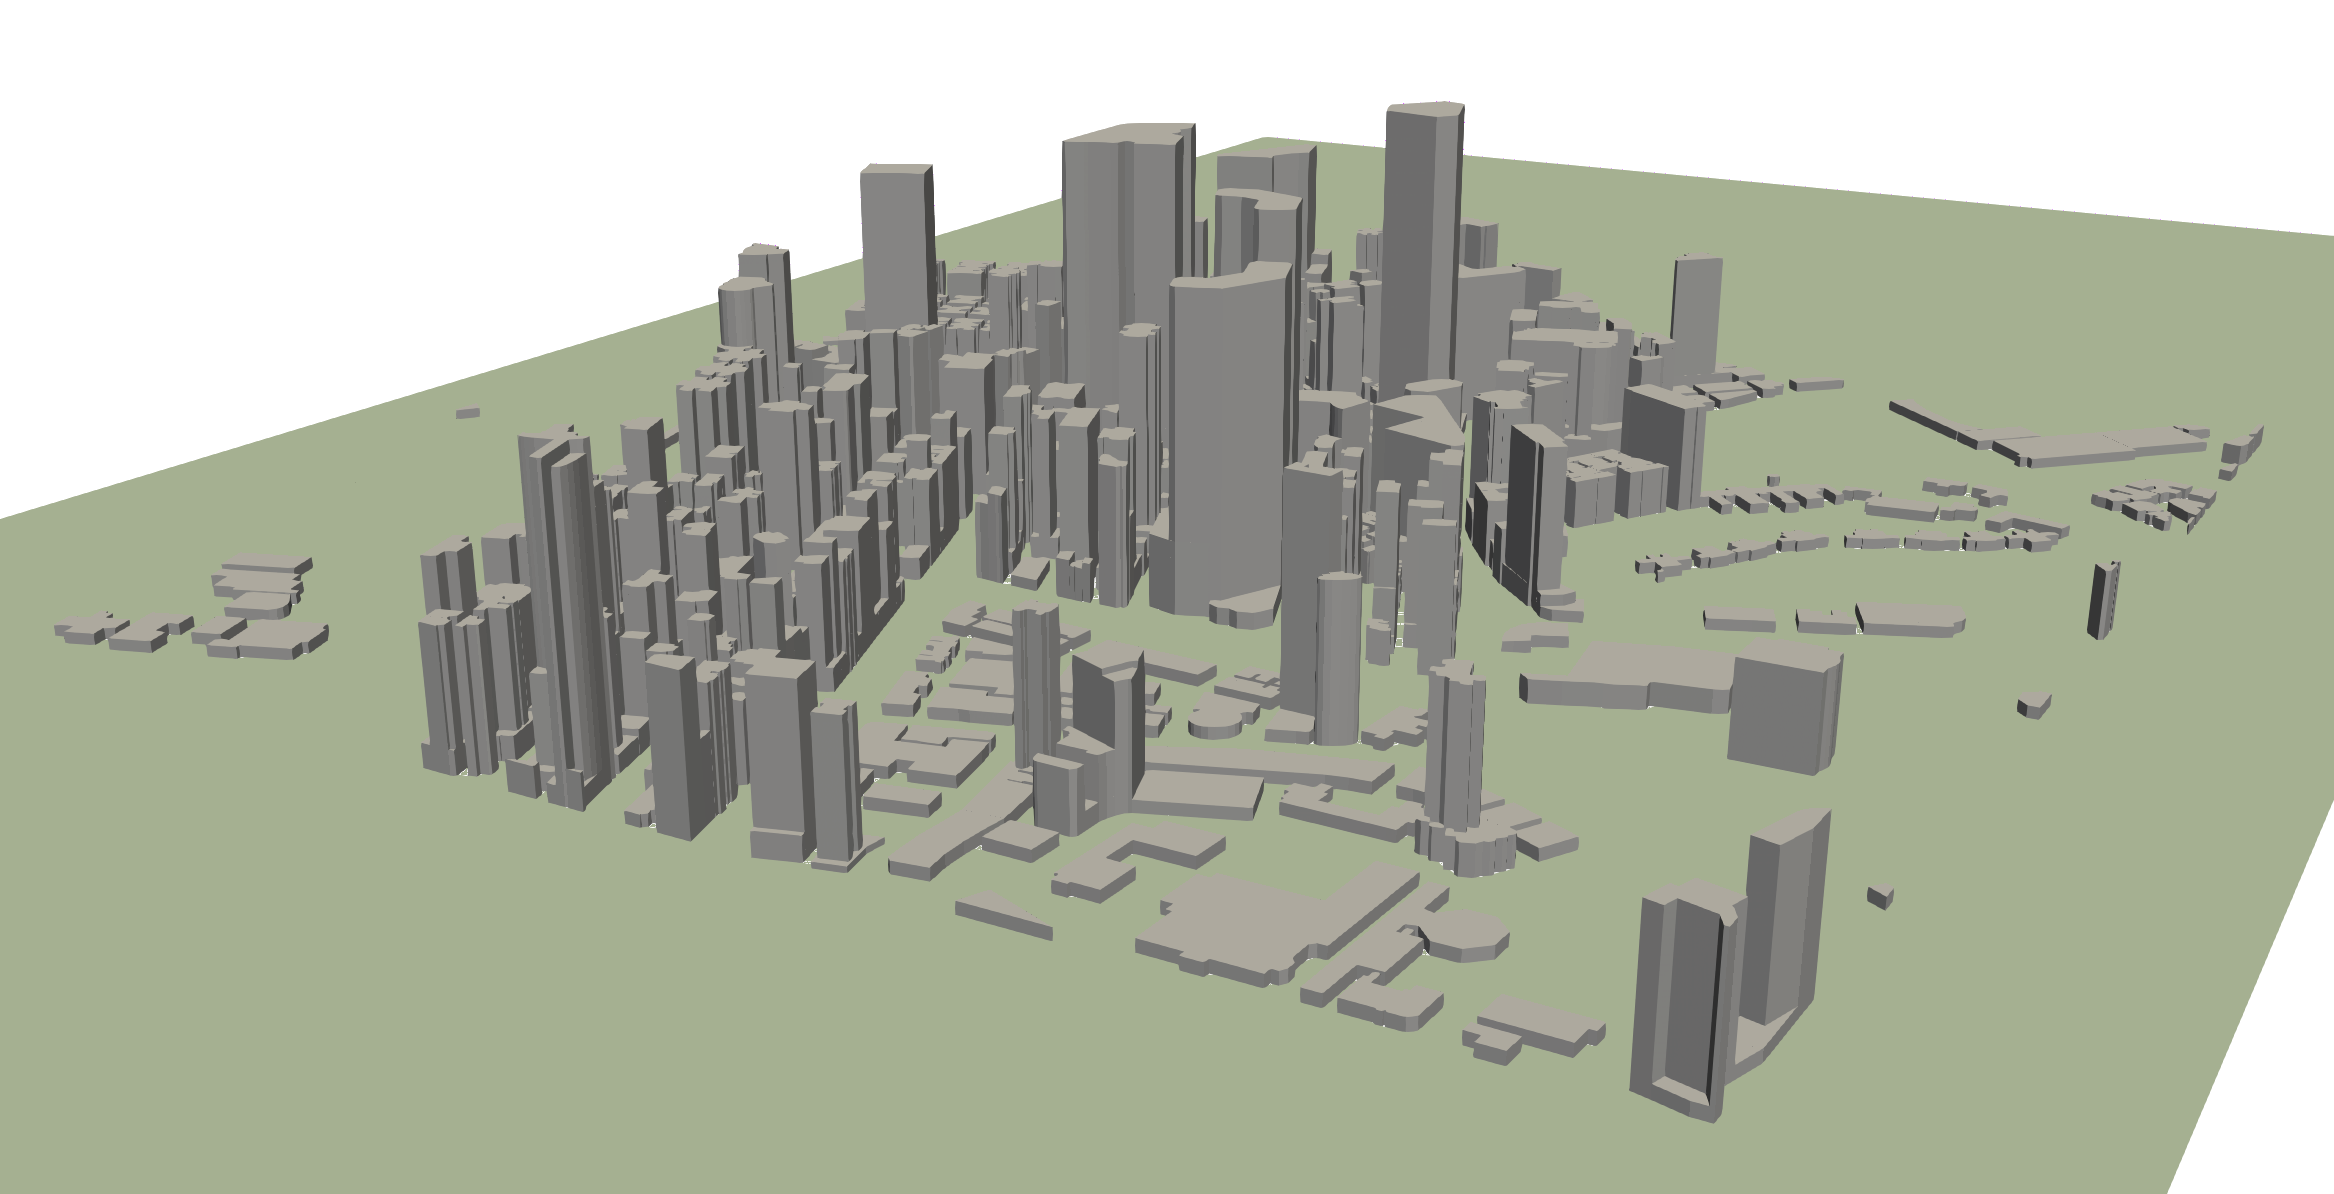
\includegraphics[width=0.95\textwidth]{01_images/geometry/geom1.png}};
        \draw[latex-latex, color=yellow, line width = 0.005\textwidth] ([yshift=0.07\textwidth,xshift=0-0.015\textwidth]obr.east) -- ([xshift=0.24\textwidth,yshift=0.025\textwidth]obr.south);
        \node at (obr.south east) [xshift=0-0.1\textwidth,yshift=0.15\textwidth] {500\,m};
        \draw[latex-latex, color=yellow, line width = 0.005\textwidth] ([xshift=0.2\textwidth,yshift=0.025\textwidth]obr.south) -- ([xshift=0.012\textwidth,yshift=0-0.03\textwidth]obr.west);
        \node at (obr.south) [xshift=0-0.2\textwidth,yshift=0.12\textwidth] {500\,m};
        \draw[-latex, color=yellow,line width = 0.005\textwidth] ([xshift=0.11\textwidth,yshift=0.09\textwidth]obr.center) -- ([xshift=0.113\textwidth,yshift=0-0.055\textwidth]obr.north);
        \node at (obr.north) [xshift=0.155\textwidth,yshift=0-0.083\textwidth] {105\,m};
        \draw (-6.5,-3.2) pic[solid] {axPic};
    \end{tikzpicture}
    \caption{Studied city geometry (used \textit{stl} file) with its dimensions and chosen Cartesian coordinate system.}
    \label{fig:geom1}
\end{figure}

\paragraph{Computational mesh} Computational mesh was prepared using the OpenFOAM \texttt{blockMesh} and \texttt{snappyHexMesh} utilities. The computational domain dimensions were determined based on the review by \citet{Pantusheva22}. In particular, we introduce both upstream, and downstream buffers in front of, and behind the city, which are in order $L_{\mathrm{CFDu}} = 5\,L_{\mathrm{h}}$, and $L_{\mathrm{CFDd}} = 10\,L_{\mathrm{h}}$ long. Furthermore, the computational domain is $L_{\mathrm{CFDh}} = 6\,L_{\mathrm{h}}$ high. The $y$-normal slices cut in the middle of the used computational mesh are shown in Figure~\ref{fig:mesh1}. Note the grading of the computational mesh in the $z$-direction, and its refinement in the vicinity of the city. 

\begin{figure}[htpb]
    \begin{tikzpicture}
        \node (obr) {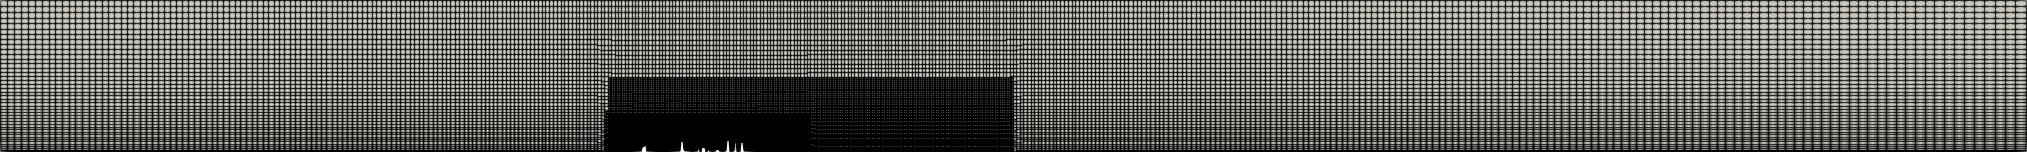
\includegraphics[width=0.95\textwidth]{01_images/geometry/mesh1.png}};
        \draw[latex-latex, line width=0.002\textwidth] ([xshift=0.005\textwidth]obr.north west)--([xshift=0-0.19\textwidth]obr.north);
        \node at (obr.north) [anchor = south west,xshift=0-0.42\textwidth] {$L_{\mathrm{CFDd}}\,=\,5\,L_{\mathrm{h}}$};
        \draw[latex-latex, line width=0.002\textwidth] ([xshift=0-0.12\textwidth]obr.north)--([xshift=0-0.005\textwidth]obr.north east);
        \node at (obr.north) [anchor = south west,xshift=0.08\textwidth] {$L_{\mathrm{CFDu}}\,=\,10\,L_{\mathrm{h}}$};
        \draw[latex-latex, line width=0.002\textwidth] ([yshift = 0-0.005\textwidth] obr.north west) -- ([yshift=0.005\textwidth] obr.south west);
        \node at (obr.west) [rotate=90,anchor = south] {$6\,L_{\mathrm{h}}$};
        \node (detail1) at (obr.south west) [inner sep=0,yshift=0-0.01\textwidth,anchor = north west,xshift=0.008\textwidth] {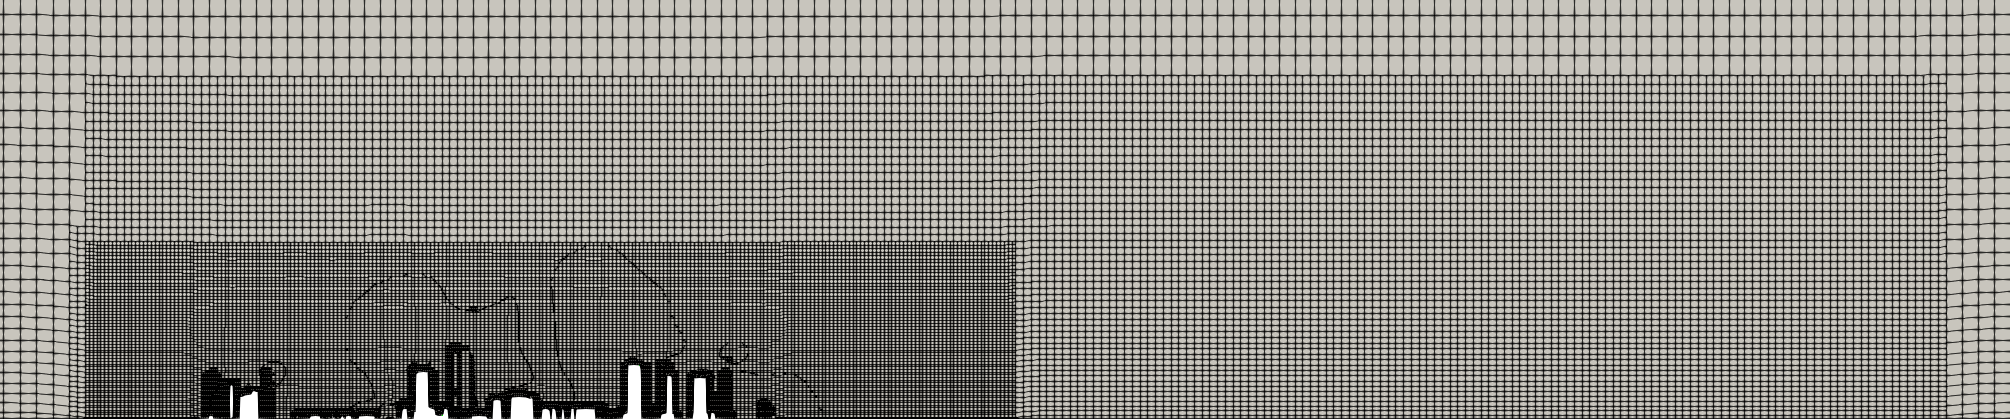
\includegraphics[width=0.45\textwidth]{01_images/geometry/mesh2.png}};
        \draw[line width = 0.003\textwidth, color=yellow!20!orange] (detail1.north west) -- (detail1.north east)--(detail1.south east) -- (detail1.south west) -- (detail1.north west);
        \draw[line width=0.003\textwidth, color=yellow!20!orange] ([xshift=0.005\textwidth,yshift=0.007\textwidth]obr.south)--([xshift=0-0.2\textwidth,yshift=0.007\textwidth]obr.south) -- ([xshift=0-0.2\textwidth,yshift=0.05\textwidth]obr.south)--([xshift=0.005\textwidth,yshift=0.05\textwidth]obr.south) --([xshift=0.005\textwidth,yshift=0.007\textwidth]obr.south);
        \node (detail2) at (obr.south east) [inner sep = 0, yshift = 0-0.01\textwidth,anchor = north east,xshift=0- 0.008\textwidth] {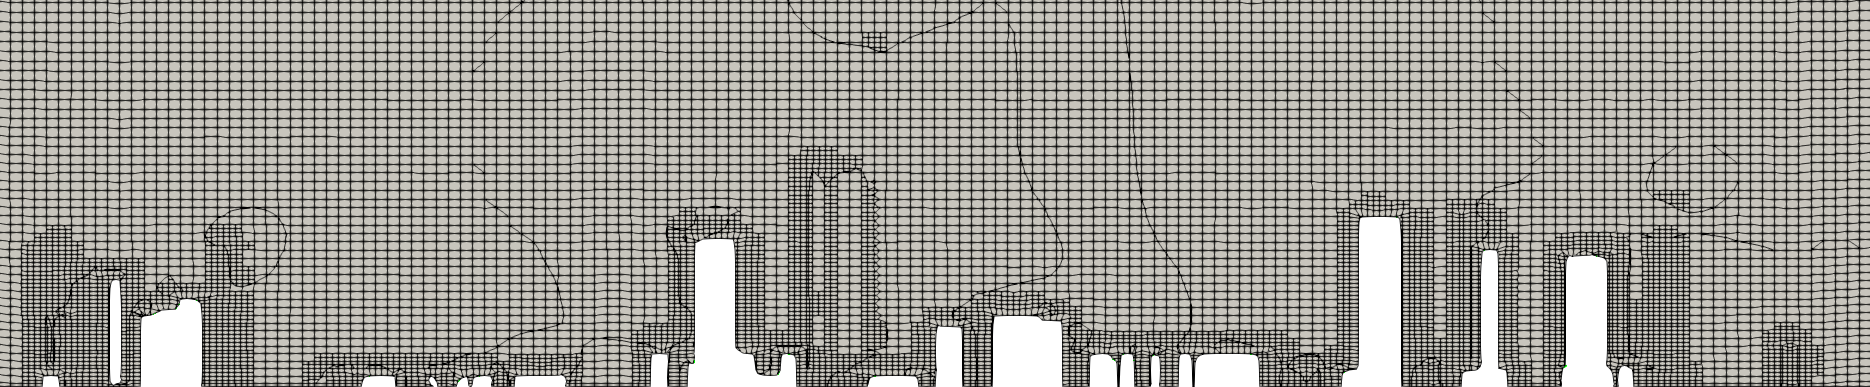
\includegraphics[width=0.45\textwidth]{01_images/geometry/mesh3.png}};
        \draw[line width = 0.003\textwidth, color=blue!70] (detail2.north west) -- (detail2.north east)--(detail2.south east) -- (detail2.south west) -- (detail2.north west);
        \draw[line width=0.003\textwidth, color=blue!70] ([xshift=0-0.12\textwidth,yshift=0.007\textwidth]obr.south)--([xshift=0-0.181\textwidth,yshift=0.007\textwidth]obr.south) -- ([xshift=0-0.181\textwidth,yshift=0.022\textwidth]obr.south)--([xshift=0-0.12\textwidth,yshift=0.022\textwidth]obr.south) --([xshift=0-0.12\textwidth,yshift=0.007\textwidth]obr.south);
    \end{tikzpicture}
    \caption{$y$-normal slices through the half of the computational mesh.}
    \label{fig:mesh1}
\end{figure}

\paragraph{Boundary conditions} The model behavior in the computational domain ($\Omega$) is described by partial differential equations outlined in the following subsection~\ref{subsec:govEq} (\nameref{subsec:govEq}). However, these need to be supplied with the consistent boundary conditions on the $\Omega$ boundary, $\partial\Omega$. As depicted in Figure~\ref{fig:bc}, the computational domain boundary is split into 
\begin{inparaenum}[(i)]
    \item \textit{inlet} ($\partial\Omega_{\mathrm{i}}$),
    \item \textit{outlet} ($\partial\Omega_{\mathrm{o}}$),
    \item \textit{ground} ($\partial\Omega_{\mathrm{g}}$),
    \item \textit{sides} ($\partial\Omega_{\mathrm{s}}$), and
    \item \textit{top} ($\partial\Omega_{\mathrm{t}}$).
\end{inparaenum}
 
\begin{figure}[htpb]
    \begin{tikzpicture}
        \node (obr) {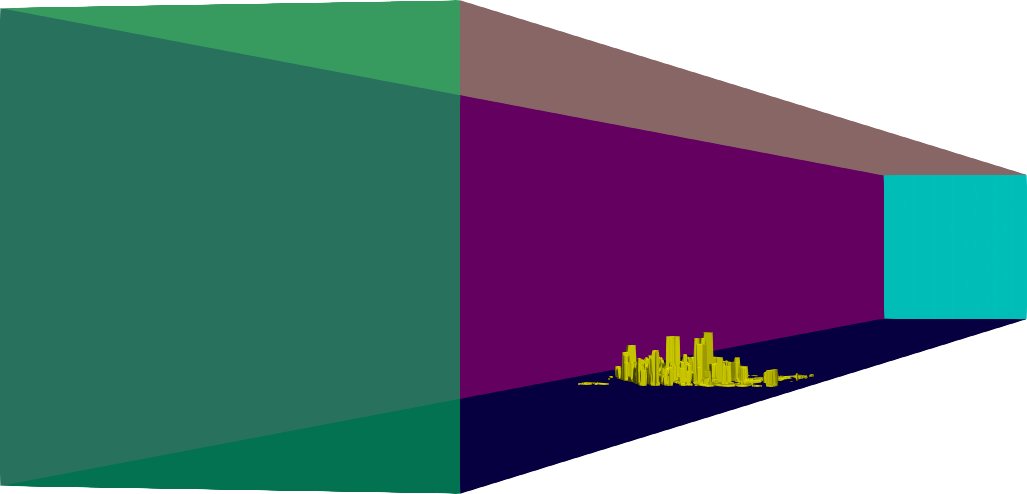
\includegraphics[width=0.5\textwidth]{01_images/geometry/bc1.png}};
        \node (inlet) at ([{shift={(0.05\linewidth,0-0.02\linewidth)}}]obr.north east) [draw,color=in,fill=in,minimum width=0.03\linewidth,minimum height=0.03\linewidth] {};
        \node [name=wall, at=(inlet.east),anchor=west]{{$\partial\Omega_{\mathrm{i}}$}};
        \node (outlet) at (inlet.south) [draw,color=out,fill=out,minimum width=0.03\linewidth,minimum height=0.03\linewidth,anchor=north,yshift=0-0.01\textwidth] {};
        \node[name=wall, at=(outlet.east),anchor=west]{{$\partial\Omega_{\mathrm{o}}$}};
        \node (ground) at (outlet.south) [draw,color=city,fill=city,minimum width=0.03\linewidth,minimum height=0.03\linewidth,anchor=north,yshift=0-0.01\textwidth] {};
        \node (ground2) at (ground.east) [draw,color=lw,fill=lw,minimum width=0.03\linewidth,minimum height=0.03\linewidth,anchor=west,xshift=0.01\textwidth] {};
        \node[name=wall2, at=(ground2.east),anchor=west]{{$\partial\Omega_{\mathrm{g}}$}};
        \node (sides) at (ground.south) [draw,color=fb,fill=fb,minimum width=0.03\linewidth,minimum height=0.03\linewidth,anchor=north,yshift=0-0.01\textwidth] {};
        \node[name=wall, at=(sides.east),anchor=west]{{$\partial\Omega_{\mathrm{s}}$}};
        \node (top) at (sides.south) [draw,color=top,fill=top,minimum width=0.03\linewidth,minimum height=0.03\linewidth,anchor=north,yshift=0-0.01\textwidth] {};
        \node[name=wall, at=(top.east),anchor=west]{{$\partial\Omega_{\mathrm{t}}$}};
        \node (pol) at (top.south) [draw,color=redpol,fill=redpol,minimum width=0.03\linewidth,minimum height=0.03\linewidth,anchor=north,yshift=0-0.01\textwidth] {};
        \node[name=wall, at=(pol.east),anchor=west]{{$\partial\Omega_{\mathrm{pol}}$}};
        \node (obr2) at (wall2.south east) [anchor=west,xshift=0.01\textwidth]{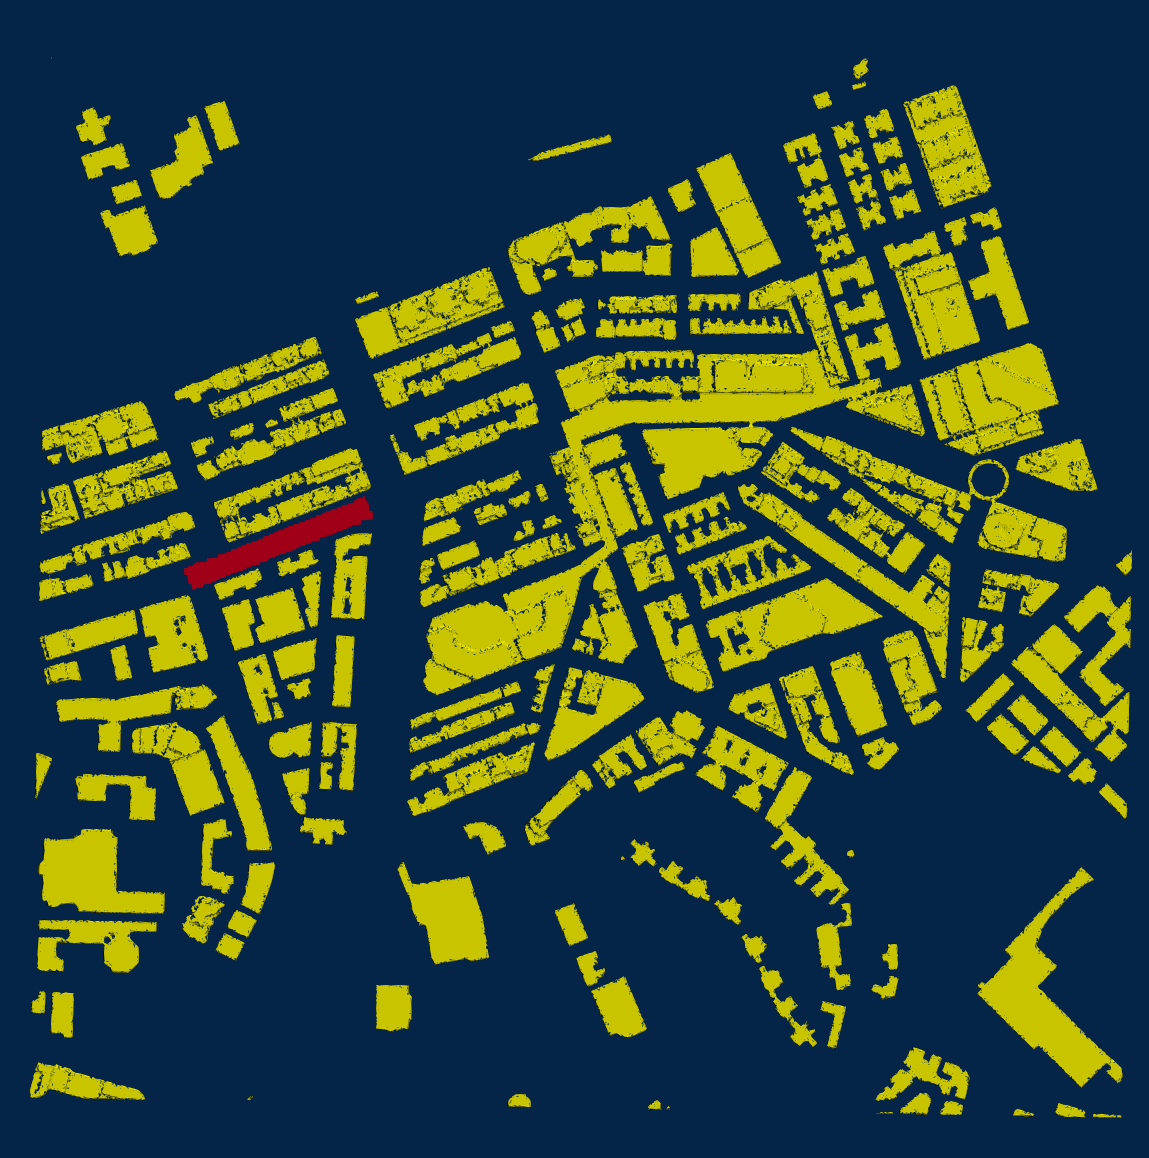
\includegraphics[width=0.25\textwidth]{01_images/geometry/bc2.png}};
        \node at (obr.north west) [anchor=south west] {a)};
        \node at (obr2.north west) [anchor=south west] {b)};
    \end{tikzpicture}
    \caption{Boundaries of the computational domain.}
    \label{fig:bc}
\end{figure}

Used boundary conditions are utilized from~\cite{kadaverugu21,Pantusheva22} and summarized in Table~\ref{tab:bc}. Starting with flow variables, uniform Dirichlet (\textit{fixedValue}), and OpenFOAM inletOutlet boundary conditions are prescribed for velocity ($\bm{u}$) at $\Omega_{\mathrm{i}}$, and $\Omega_{\mathrm{o}}$, respectively. At $\Omega_{\mathrm{g}}$, we standardly assume \textit{noSlip} boundary condition, and finally the sides of the geometry ($\Omega_{\mathrm{s}}$ and $\Omega_{\mathrm{t}}$) are treated as the symmetry (\textit{slip}). This setting is supplemented with OpenFOAM \textit{totalPressure} boundary condition for pressure ($p$) at $\Omega_{\mathrm{o}}$, and zeroGradient (\textit{zeroGrad}) elsewhere. 

As described in the later subsection, $k-\varepsilon$ turbulence model is used to estimate unresolved eddy dissipation. The turbulence model requires specification of the boundary conditions for turbulent kinetic energy ($k$), rate of dissipation of the turbulent kinetic energy ($\varepsilon$), and the turbulent viscosity ($\nu_{\mathrm{t}}$). At $\Omega_{\mathrm{i}}$, we use OpenFOAM turbulentIntensityKineticEnergyInlet (\textit{turbIntKinEngInlet}), and turbulentMixingLengthDissipationRateInlet (\textit{turbMixDissRateInlet}) boundary conditions, which calculate the inlet $k$ and $\varepsilon$, respectively, based on specified value of the inlet turbulence intensity $I_{\mathrm{i}}$. At the $\Omega_{\mathrm{g}}$, standard wall functions are utilized \textit{kqRWallFunction}, \textit{epsWallFunction}, and \textit{nutkWallFunction}, in order for $k$, $\varepsilon$, and $\nu_{\mathrm{t}}$. And finally, \textit{zeroGrad} boundary condition is prescribed elsewhere.

Scalar transport equation describing the spreading of the pollution $y_{\mathrm{P}}$ is supplied with the \textit{fixedValue} boundary condition at $\Omega_{\mathrm{g}}$, defining the source of the pollution on the main road, and \textit{zeroGrad} boundary condition elsewhere.

\begin{table}[htbp]
    \caption{Used boundary conditions.}
    \label{tab:bc}
    \centering
    {
    \begin{tabular}{lccccccccc}
        \hline
        variable & $\Omega_{\mathrm{i}}$ & $\Omega_{\mathrm{o}}$ & $\Omega_{\mathrm{g}}$ &  $\Omega_{\mathrm{s}}$ & $\Omega_{\mathrm{t}}$ \\
        \hline
        $\bm{u}$ & fixedValue & inletOutlet & noSlip & slip & slip\\
        $p$ & zeroGrad & totalPressure & zeroGrad & zeroGrad & zeroGrad\\
        $k$ & turbIntKinEngInlet & zeroGrad & kqRWallFunction & zeroGrad & zeroGrad\\
        $\varepsilon$ & turbMixDissRateInlet & zeroGrad & epsWallFunction & zeroGrad & zeroGrad\\
        $\nu_{\mathrm{t}}$ & fixedValue & zeroGrad & nutkWallFunction & zeroGrad & zeroGrad\\
        $y_{\mathrm{P}}$ & zeroGrad & zeroGrad & fixedValue & zeroGrad & zeroGrad\\
        \hline
    \end{tabular}
    }
\end{table}

\subsection{Governing equations}
\label{subsec:govEq}
The description of the chosen governing equations is split into two parts, 
\begin{inparaenum}[(i)]
    \item air-flow governing equations, and
    \item the pollution scalar transport.
\end{inparaenum}

\paragraph{Flow governing equations} Steady state isothermal incompressible flow of the Newtonian gas is assumed. Adopting Boussinesq hypothesis, and noting the mean time velocity, $\bm{u}\,=\,(u_x,u_y,u_z)^\intercal$, and the mean time turbulent pressure, $\tilde{p}$, the flow can be described by Reynolds-averaged Navier-Stokes (RANS) equations in a form,
\begin{align}
    \label{eq:RANS1}
    \nabla\cdot(\bm{u}\bm{u}^\intercal) - \nabla\cdot\left[(\nu + \nu_{\mathrm{t}})\,(\nabla \bm{u} + (\nabla\bm{u})^\intercal)\right] &= - \nabla \tilde{p}\,,\\
    \label{eq:RANS2}
    \nabla\cdot(\bm{u}) &= 0\,
\end{align}
where $\nu$ is the gas kinematic viscosity, and $\nu_{\mathrm{t}}$ is the turbulent eddy viscosity.

In general, there exist numerous various approaches of $\nu_{\mathrm{t}}$ estimation. In the present work, the OpenFOAM variant of $k-\varepsilon$ turbulence model is used to calculate the turbulent eddy viscosity as,
\begin{equation}
    \label{eq:nut}
    \nu_{\mathrm{t}} = \frac{k}{\varepsilon}\,,
\end{equation}
where $k$, and $\varepsilon$ are the turbulence kinetic energy, and its rate of the dissipation, respectively. For more information on the calculation of the $k$ and $\varepsilon$, see e.g.~\cite{moukalled16,launder1974}.

\paragraph{Pollution transport governing equation} Assuming constant mass density, the transient dispersion of the polluting gas in the carrier gas can be estimated employing standard scalar variable transport equation in a form,
\begin{equation}
    \label{eq:scTr}
    \frac{\partial (y_{\mathrm{P}})}{\partial t} + \nabla\cdot(\bm{u}\, y_{\mathrm{P}}) - \nabla\cdot((D\,+\,D_{\mathrm{t}}) \nabla y_{\mathrm{P}}) = 0\,,
\end{equation}
where $\bm{u}$ is the mean-time velocity obtain from solution of~(\ref{eq:RANS1},\ref{eq:RANS2}), $y_{\mathrm{P}}$ is the molar fraction of the polluting gas, $t$ is time, and $D$ and $D_{\mathrm{t}}$ are in order molar and turbulent diffusivities of the polluting gas. Remark that no source of the pollution is assumed on the right hand side of the equation~\eqref{eq:scTr}, as the source of the pollution is ensured by proper application of the boundary conditions.

Furthermore, the turbulent diffusivity, $D_{\mathrm{t}}$, is calculated using Schmidt number (Sc) defined as, 
\begin{equation}
    \label{eq:Sc}
    \mathrm{Sc} = \frac{\nu + \nu_{\mathrm{t}}}{D + D_{t}}\,,
\end{equation}
where $\nu + \nu_{\mathrm{t}}$ are the gas kinematic and the turbulent viscosities, respectively. Note that a standard assumption of the constant Schmidt number is adopted~\cite{baik03}, and $\nu_{\mathrm{t}}$ is estimated from from~\eqref{eq:nut}.

\subsection{Model parameters}
\label{subsec:modPars}
The above described mathematical model has several tunable parameters that can be split into two groups,
\begin{inparaenum}[(i)]
    \item thermophysical parameters of the flowing gas, and
    \item boundary conditions
\end{inparaenum}

The flow of the air at the common temperature of the $T\,=\,25\,^\circ$C has been assumed. The value of the gas kinematic viscosity has been calculated from Sutherland equation~\cite{sutherland1893} as $\nu$ = 1.53$\,\cdot\, 10^{-5}\,\mathrm{m^2\,s^{-1}}$, and the value of the pollution molar diffusivity from Fuller equation~\cite{fuller66} as $D$ = 1.72$\,\cdot\, 10^{-5}\,\mathrm{m^2\,s^{-1}}$.  As in~\cite{baik03}, the Schmidt number has been assumed constant and equal Sc$\,=\,0.9$.

To complete the description of the prepared model, it remains to specify the inlet values of the velocity, and the turbulence intensity, and the value of the pollution molar fraction on the ground of the main road (see $\partial\Omega_{\mathrm{pol}}$ in Figure~\ref{fig:bc}b on page~\pageref{fig:bc}). For the case of the tutorial example, we have prescribed $u_{\mathrm{in}}$ = 10\,$\mathrm{m\,s^{-1}}$, $I_\mathrm{i}$ = 5\,\%, and $y_{\mathrm{pol,\partial\Omega_{\mathrm{pol}}}}$ = 10\,\%.